\documentclass[a4paper,ngerman]{scrartcl}

\usepackage{amsmath}
\usepackage{amsfonts}
\usepackage{amssymb}
\usepackage[utf8]{inputenc}
\usepackage{graphicx}
\usepackage[ngerman]{babel}
\usepackage{hyperref}
\usepackage{float}
\usepackage{caption}
\usepackage{subcaption}
\usepackage{multirow}  %for tables
\usepackage{icomma} % Handle german comma as decimal point in numbers
\usepackage{units,siunitx} % Write units with correct spacing
\usepackage{upgreek} % provide non-italic greek letters
\usepackage{url}
\usepackage{hepnames} % hier gibt es symbole fuer unterschiedliche elementarteilchen, aber dieses paket gibts nicht im poolraum

%\usepackage{subfig}

% Formatting of table & figure captions
\captionsetup{font={sf,footnotesize},labelfont=bf,textfont=sl,skip=6pt}

\sisetup{locale = DE, % use "," as decimal point instead of "."
  exponent-product={\cdot},% used \cdot in front of 10^x
  separate-uncertainty} % give out uncertainty with \pm instead of in brackets

\setlength{\abovecaptionskip}{6pt}
\setlength{\belowcaptionskip}{0pt}

\title{Elementarteilchen 2\\Vorbereitung}
\date{\today}
\author{Michel Rausch, Michael Eliachevitch}

\begin{document}

\maketitle
\tableofcontents
\newpage

\section{Einleitung}

Nach dem Standartmodell (\textbf{SM}) der Teilchenphysik gibt es zwei große Gruppen der Elementarteilchen.
Eine werden Fermionen genannt und besitzen einen Spin von $\frac{1}{2}$. 
Zu ihnen gehören beispielsweise Elektronen.
Die andere Gruppe sind die Bosonen mit einem Spin von $1$.

Fermionen sind weiterhin gegliedert in Leptonen und Quarks.
Des weiteren sind sie in 3 Generationen unterteilt aus jeweils zwei Quarks und zwei Leptonen. 
Eine Übersicht der Fermionen ist in Abbildung \ref{fig:fermionen} gezeigt.
Up- und Down-Quarks bilden mit Elektronen die Grundlage für gewöhnliche Materie.
\begin{figure}[tbh!]
\centering
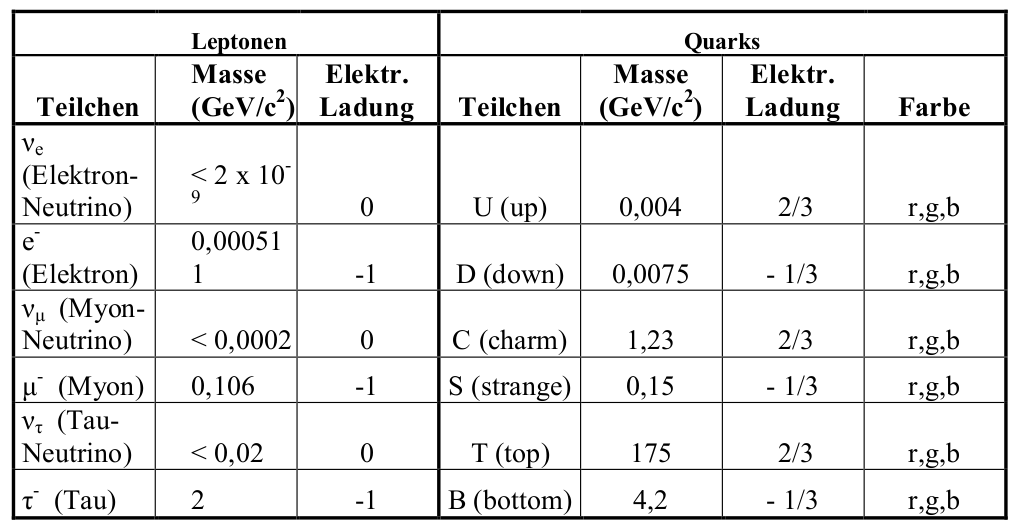
\includegraphics[width=0.7\textwidth]{abbildungen/fermionen.png}
\caption{\textbf{Eigenschaften der Fermionen [\ref{ref:BB}].} 
}
\label{fig:fermionen}
\end{figure}

Zwischen Teilchen gibt es Wechselwirkungen.
Im SM werden die Kräfte mit einem Austausch von Teilchen, den Austausch- oder Eichbosonen erklärt.
Das Photon ist das masselose Eichboson der elektromagnetischen Wechselwirkung.
Die schwache Wechselwirkung besitzt die massiven Vektorbosonen \PWpm , sowie \PZzero als Eichbosonen.
Gluonen gehören zur starken Wechselwirkung.
Das postulierte Graviton für die Gravitationskraft konnte noch nicht nachgewiesen werden.
Eine Übersicht der Bosonen mit ihren Wechselwirkungen befindet sich in Abbildung \ref{fig:bosonen}.
Als Erweiterung des SM gibt es den Higgs-Mechanismus.
Das vorausgesagte Higgs-Boson wurde durch den Nachfolger des LEPs, dem LHC, gefunden.

\begin{figure}[tbh!]
\centering
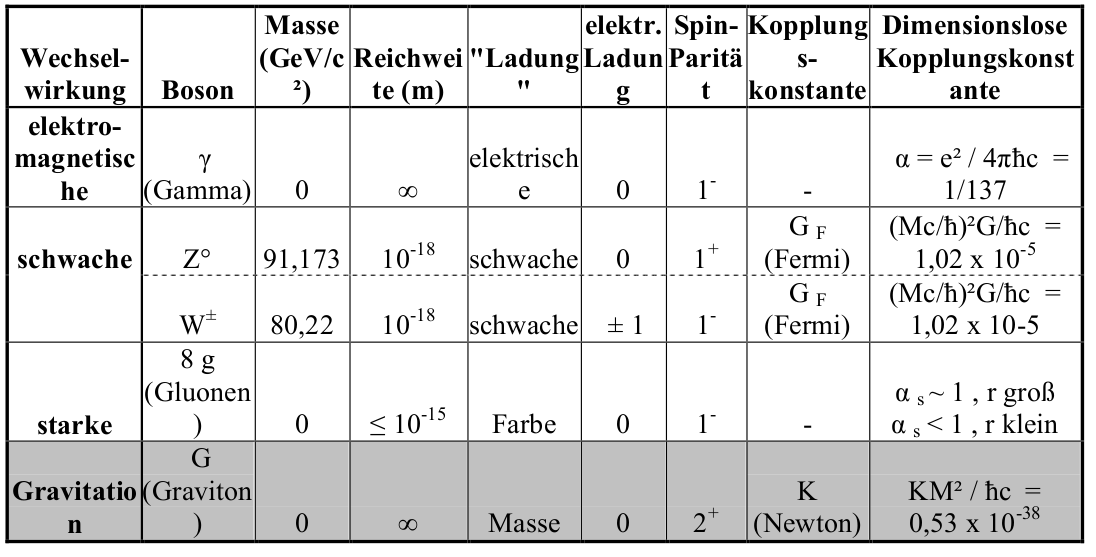
\includegraphics[width=0.7\textwidth]{abbildungen/bosonen.png}
\caption{\textbf{Eigenschaften der Bosonen und der zugehörigen Wechselwirkung~[\ref{ref:BB}].} 
}
\label{fig:bosonen}
\end{figure}

Diese Teilchen lassen sich in einem Teilchenbeschleuniger erzeugen und untersuchen.
In diesem Versuch werden die Eigenschaften einiger Teilchen untersucht anhand der Daten des DELPHI. 
Auch die Wechselwirkung zwischen Elementarteilchen wird untersucht.
Die Funktionsweise eines Detektors, sowie die Auswertung der entstandenen Daten soll mit diesem Experiment verständlich gemacht werden.



\section{Das DELPHI Experiment am LEP}
\label{sec:delphi}

Der LEP (Large Electron Positron) Collider war ein Teilchenbeschleuniger des CERN.
Er befand sich nahe Genf \SI{100}{\metre} unter der Erde und war \SI{27}{\kilo \metre} lang [\ref{ref:hands-on}]. 
Mittlerweile ist er vom Large Hadron Collider (LHC) ersetzt worden.

An vier Stufen wurden Elektronen und Positronen in entgegengesetzte Richtung auf Energien bis zu \SI{100}{GeV}~[\ref{ref:hands-on}] beschleunigt.
Die Strahlen treffen an vier Orten mit einer Schwerpunktenergie von über 200\,Gev zusammen.
Dort befinden sich Detektoren, um die Kollisionen zu analysieren, darunter der DELPHI (Detector with Lepton, Photon and Hadron Identification), der schematisch in Abbildung~\ref{fig:delphi_big} gezeigt ist.

\begin{figure}[tbh!]
\centering
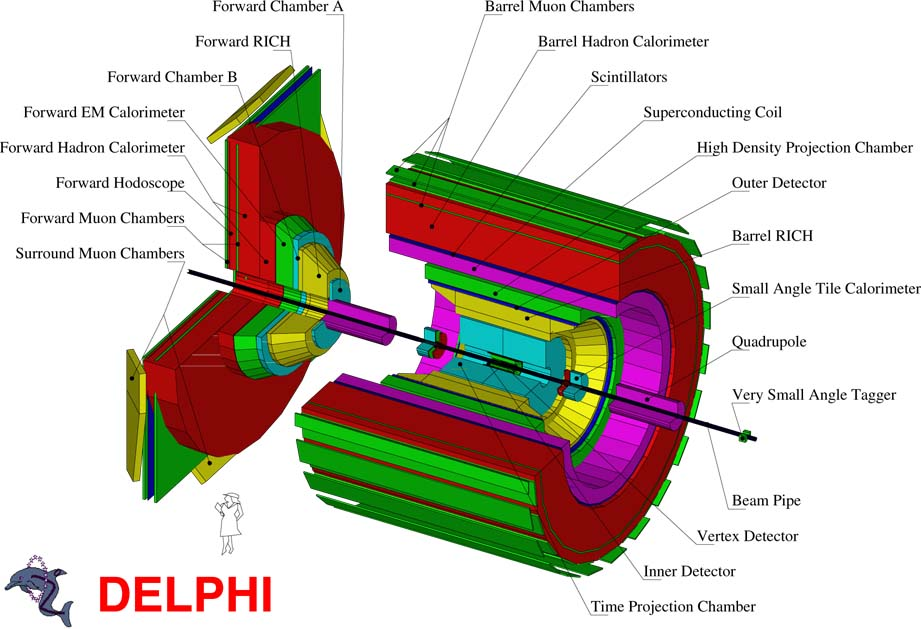
\includegraphics[width=\textwidth]{abbildungen/delphi_big.png}
\caption{\textbf{Aufbau des DELPHI-Detektors mit einer sichtbaren Endkappe~[\ref{ref:hands-on}].} 
Die Bestandteile des Detektors sind farblich gekennzeichnet und benannt.
Links ist eine der beiden Endkappen zu sehen, die andere wurde zur Übersichtlichkeit ausgeblendet.
Rechts im Bild ist der zylindrische zentrale Teil mit Strahlengang gezeigt. 
}
\label{fig:delphi_big}
\end{figure}

Der Detektor ist in Schichten aufgebaut, wie in Abbildung~\ref{fig:delphi_schichten} dargestellt ist.
Ein Magnetfeld durchströmt den gesamten Detektor und lenkt geladene Teilchen auf ihrem Weg ab, wodurch sie sich identifizieren lassen.
Die Schichten sind verschiedene Subdetektoren. 
Als innerste Schicht wird eine Spurkammer verwendet.
Einige Teilchen sind in dieser sichtbar, wie Myonen, Elektronen, oder Pionen.
Photonen und Neutronen sind aufgrund ihrer geringen Wechselwirkung hier nicht sichbar.

Als zweite Schicht wird ein Elektromagnetisches Kalorimeter (\textbf{ECAL}) verwendet.
Teilchen mit elektromagnetischer Wechselwirkung, wie Elektronen, oder Photonen werden in diesem sichtbar.
In dem ECAL entsteht eine Kaskadenschauer beim Eintritt der Elektronen und Photonen, an der diese Teilchen die gesamte Energie verlieren. 
Die schwereren Myonen passieren jedoch nahezu ungehindert.

Hadronen werden im Hadronkalorimeter (\textbf{HCAL}) abgebremst und bilden dort eine Kaskadenschauer.
Myonen passieren auch ungehindert und gelangen in die Myonkammern, wo sie detektiert werden.

Produkte der Kollision kann man anhand dieses Schemas erkennen. 
Wenn ein Jet beispielsweise nicht in der Spurkammer sichtbar ist, aber im ECAL seine Energie verliert und eine Kaskade auslöst,
so handelt es sich dabei höchstwahrscheinlich um ein Photon.
Damit lässt sich anhand geeigneter Darstellungsmethoden und Software, wie in Kapitel~\ref{sec:scannen} beschrieben ist, die Ergebnisse aus den Detektoren analysieren.

\begin{figure}[tbh!]
\centering
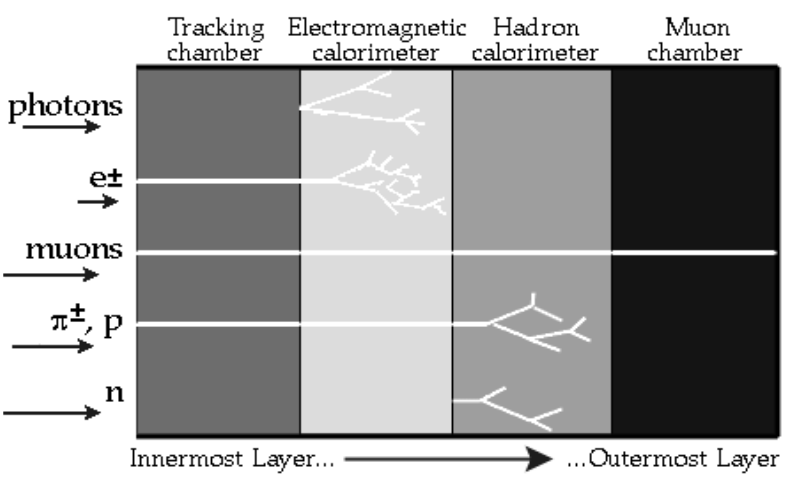
\includegraphics[width=0.7\textwidth]{abbildungen/delphi_schichten.png}
\caption{\textbf{Übersicht der Signaturen nachweisbarer Teilchen in den Subdetektoren~[\ref{ref:BB}].} 
Photonen durchqueren die Spurkammer und werden erst im ECAL detektiert.
Elektronen und Positronen bilden Spuren in der Spurkammer und verlieren ihre Energie im ECAL.
Myonen bilden Spuren bis in die Myonkammer.
Hadronen lösen verlieren ihre Energie im HCAL.
Neutronen bilden keine Spur in der Spurkammer und sind nicht im ECAL sichtbar, da sie keine Ladung besitzen.
Protonen und geladene Pionen hingegen sind in der Spurkammer, sowie im ECAL sichtbar.
}
\label{fig:delphi_schichten}
\end{figure}


%\section{Mögliche Zerfälle und Bestimmung der Zerfallsbreiten und Kopplungskonstanten}
\section{Theoretische Betrachtung unterschiedlicher Zerfälle}
\label{sec:zerfaelle}

Wie bereits in Kapitel~\ref{sec:delphi} angesprochen, wurden im LEP \Pelectron-\APelectron-Paare zur Kollision gebracht, wobei gegen Ende Schwerpunktsenergien von über 200\,Gev~\ref{ref:cernlep} erreicht wurden,
womit neue Teilchen erzeugt werden konnten.
Dabei konnten neue Teilchen entstehen, 
solange diese die Erhaltungssätze des Standardmodells nicht verletzen 
und deren Energie nicht die Schwerpunktsenergie der Kollision übersteigt.
Aufgrund der Erhaltung der elektrischen Ladung und der Farbladung, 
die beide in der Summe bei dem \Pelectron-\APelectron-Paar null sind,
entstand bei einer Kollision immer zuerst eines der beiden neutralen Eichbosonen,
nämlich entweder ein Photon oder ein \PZzero-Boson,
welches eine Ruhemasse von 91\,GeV~\ref{ref:BB} besitzt.
Beides sind virtuelle Teilchen, die schnell in weitere Teilchen zerfallen,
weshalb aufgrund der Unschärferelation die Masse des virtuellen
Teilchens die Energieerhaltung auch verletzen kann.
Wir werden in diesem Versuch die Zerfälle des \PZzero-Bosons betrachten.\\

Die virtuellen Eichbosonen können in Leptonen-Antileptonen- oder auch 
Quark-Antiquark-Paare unterschiedlicher Teilchenfamilien zerfallen. 
Die Teilchen der schwereren Teilchenfamilien sind instabil und zerfallen weiter in leichtere Teilchen.
Bei Quarks ist zu beachten, dass diese nicht frei existieren können,
da die starke Kernkraft bei zunehmendem Abstand zunimmt.
Durch die große potentielle Energie bilden sich neue Quark-Antiquark-Paare,
bis am Ende nur noch gebundene Zustände Quarks vorhanden sind. 
Dabei handelt es sich um 
Mesonen aus Quark und Antiquark mit entgegengesetzter Farbladung und um Hadronen aus 3 Quarks,
in denen jede Farbladung vorhanden ist. 
Dabei entstehen sogenannte Jets. 
Es gibt immer mindestens zwei davon, da das \PZzero zuerst in ein Quark-Antiquark-Paar zerfällt. 
Dann spricht man von 2-Jets.
Oft gibt es auch drei Jets, sogenannte 3-Jets, wobei der dritte Jet durch Gluonabstrahlung entsteht,
welches wie die Quarks eine Farbladung hat und damit der starken Wechselwirkung unterliegt und folglich ebenfalls Jets erzeugt.
Die Entstehung eines 3-Jets aus dem Zerfall eines in einer \Pelectron-\APelectron-Kollision entstandenen \PZzero-Bosons ist 
in dem Feynmandiagramm in Abbildung~\ref{fig:3jet} gezeigt.
Da das Gluon mit der starken Kraft an das Quark koppelt, ist die
Wahrscheinlichkeit eines 3-Jets proportional zur
Kopplungskonstante der starken Kernkraft.\\
\begin{figure}[tbh!]
  \centering
  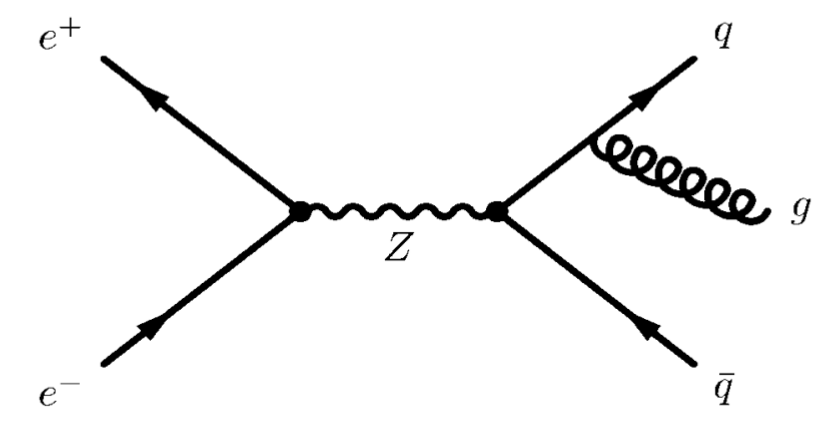
\includegraphics[width=0.7\textwidth]{abbildungen/3jet_feyn.png}
  \caption{Entstehung eines 3-Jets im LEP.\\ Bei der Kollision von Positron und Elektron bildet sich ein virtuelles \PZzero, welches in ein Quark-Antiquark-Paar zerfällt, die beide einen Jet erzeugen. Durch die Abspaltung eines Gluons bildet sich ein dritter Jet.}
  \label{fig:3jet}
\end{figure}

Der dritte Jet bei einem 3-Jet-Ereignis zeigt in eine ähnliche Richtung wie der Jet, von dem das Gluon abgestrahlt wurde
und lässt sich daher nicht immer auflösen.
Als Bedingung für die Auflösung von zwei Jets definiert man, dass deren invariante Masse $M_{ij}$, 
die von den Jetenergien $E_i$ und $E_j$ und dem Winkel zwischen den Jets $\theta_{ij}$ abhängt,
normiert mit der Schwerpunktsenergie des Ereignisses $\sqrt s$, 
im Quadrat über einem bestimmten Wert liegen muss, den man als Jetauflösungsparameter $y_{\rm cut}$ bezeichnet.
Zwei Jets können also aufgelöst werden, wenn gilt:
\begin{equation}
  \frac{M_{ij}^2}{s} = \frac{2 E_i E_j (1-\cos \theta_{ij})}{s} > y_{\rm cut}~.
\end{equation}








\section{Das Scannen von Ereignissen mit "`Fireworks"' und Beispielzerfälle}
\label{sec:scannen}

\section{Quellen}
\begin{enumerate}
\item Blaues Buch \label{ref:BB}
\item \url{http://home.web.cern.ch/about/accelerators/large-electron-positron-collider}
 (\today) \label{ref:cernlep}
% Quelle fuer PDG-Angaben: (noch nicht genutzt, daher auskommentiert)
% \item K.A. Olive et al. (Particle Data Group), Chin. Phys. C, 38, 090001 (2014). \label{ref:pdg14}
\item \url{http://hands-on-cern.physto.se/hoc_v21en/index.html} (\today)\label{ref:hands-on}
\end{enumerate}



\end{document}
